\subsubsection{Oscillators}

Oscillators serve the foundation of synthesizer and sound design, by producing
simple waveforms, including complex wavetables. For example, the following equation describes a sine wave
expressed in terms of the sampling frequency, $f_s$.

\begin{equation}\label{eq:osc_basic_sine}
    x[n] = sin(2 \pi p),   \qquad  p = \frac{f n}{f_s}
\end{equation}

Where $f$ is the the frequency, and $p$ is the phase associated with it, and $0 \leq p \leq 1$.
This means that everytime the waveform is produced, the oscillator sends those samples into the
buffer for rendering. And as the process continues, the phase keeps incrementing, until $p = 1$, eventually
starting over. This creates periodic waveforms, therefore comprising an oscillator. And lastly, the larger
the frequency, the faster it takes to create one revolution of a signal, leading to higher pitch. The complete 
oscillator code is included in \Cref{app:synth_Code}, Listing \ref{lst:oscshape} and \ref{lst:osc_generate}.

To verify if the code produced the sine wave of frequency of 523.53 Hz and an amplitude of 0.8 linear units, 
the 5-second waveform is exported to a WAV file, and then analyzed using Audacity. The following screenshot 
in \Cref{fig:sine_wave_example} show the sine wave in the time domain, which produced the expected result.

\begin{figure}[ht]
  \centering
  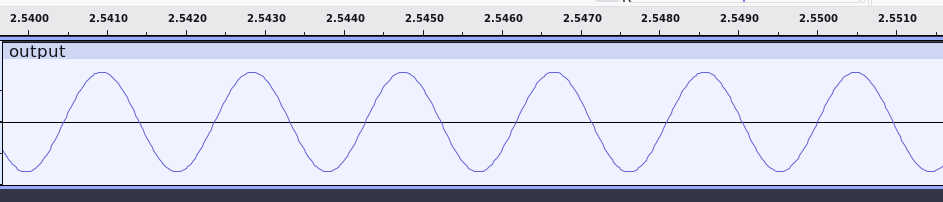
\includegraphics[width=\linewidth]{discussion/synth/figures/sine_wave_example.png}
  \caption{Sine waveform displayed in the time domain}
  \label{fig:sine_wave_example}
\end{figure}

In Fourier Analysis, sound waves are created using a collection of sine waves producing a distinct
timbre. The screenshot in \Cref{fig:sine_fft_example} shows the frequency spectrum of the same sine 
wave as mentioned above. This measured a peak frequency at \SI{528}{\hertz} ($\approx$ \SI{523.53}{\hertz}), 
and an amplitude of \SI{-1.6}{\decibel}, which is 0.832 linear units ($\approx$ 0.8).

\begin{figure}[ht]
  \centering
  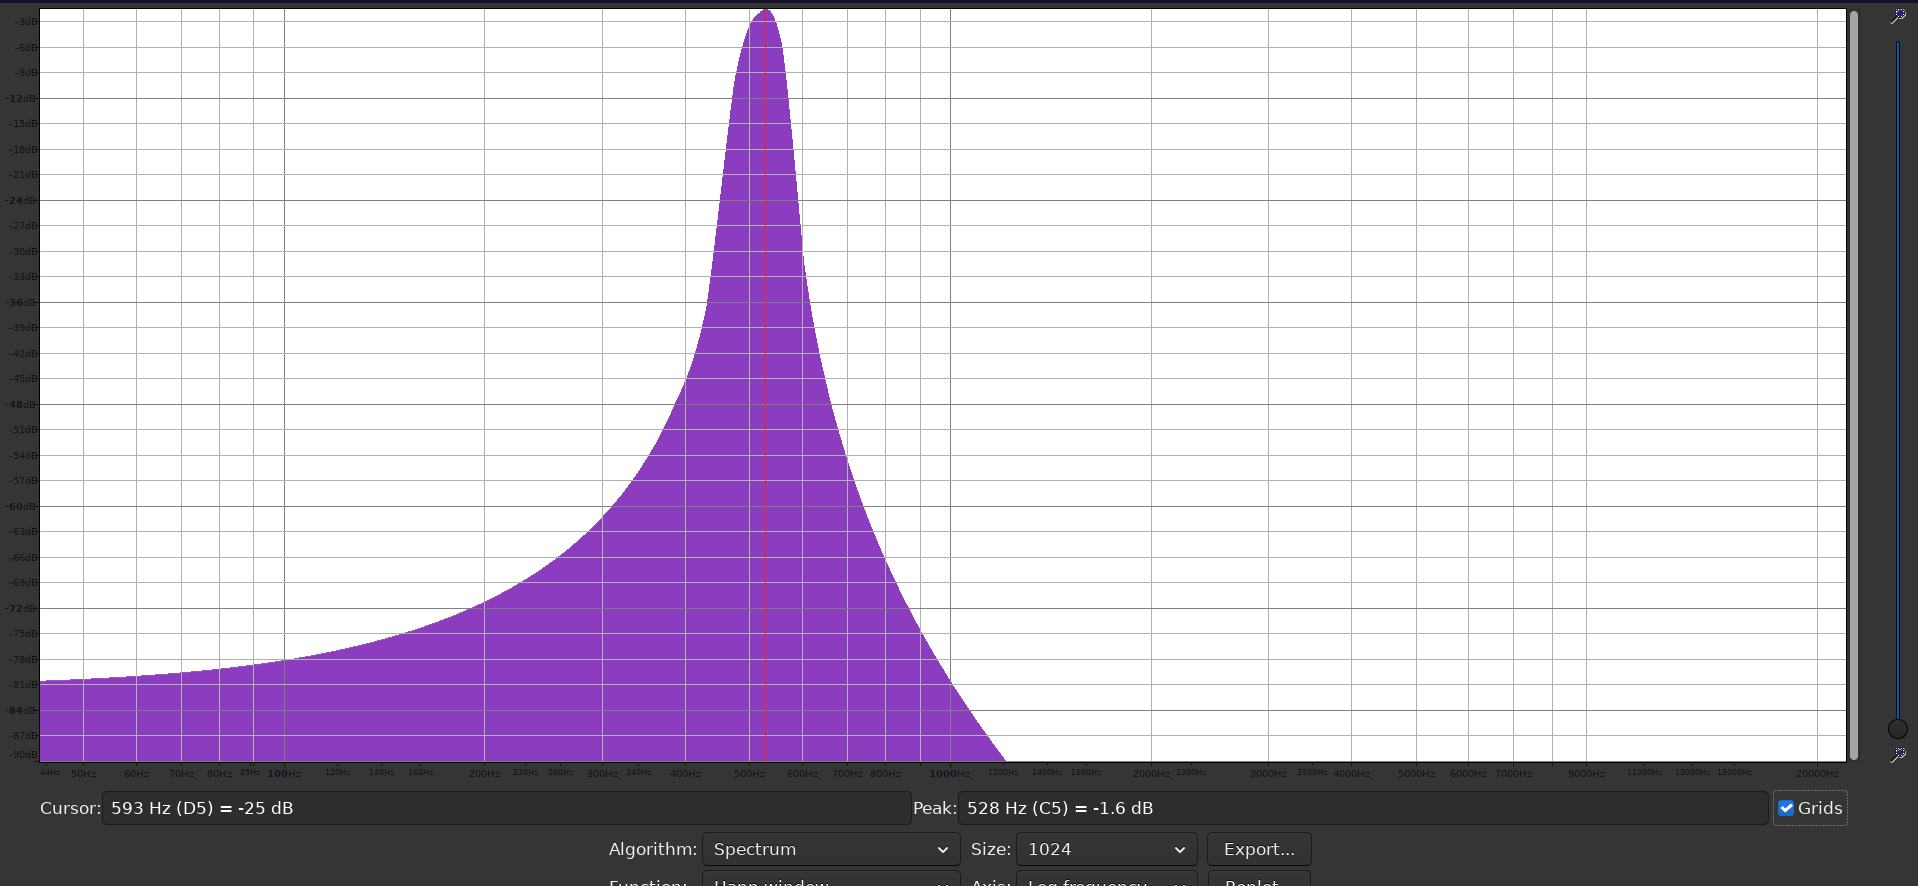
\includegraphics[width=\linewidth]{discussion/synth/figures/sine_fft_example.png}
  \caption{Frequency spectra of a sine wave showing a single harmonic peak}
  \label{fig:sine_fft_example}
\end{figure}

To verify that an oscillator generated patterns more complex than sine, the frequency spectrum
of the generated sawtooth wave (\SI{220}{Hz}) is analyzed and compared with the literature 
\cite{wilczek2022waveforms} as shown in \Cref{fig:saw_spectrum}.

\begin{figure}[ht]
  \centering
  \begin{minipage}[b]{0.48\linewidth}
    \centering
    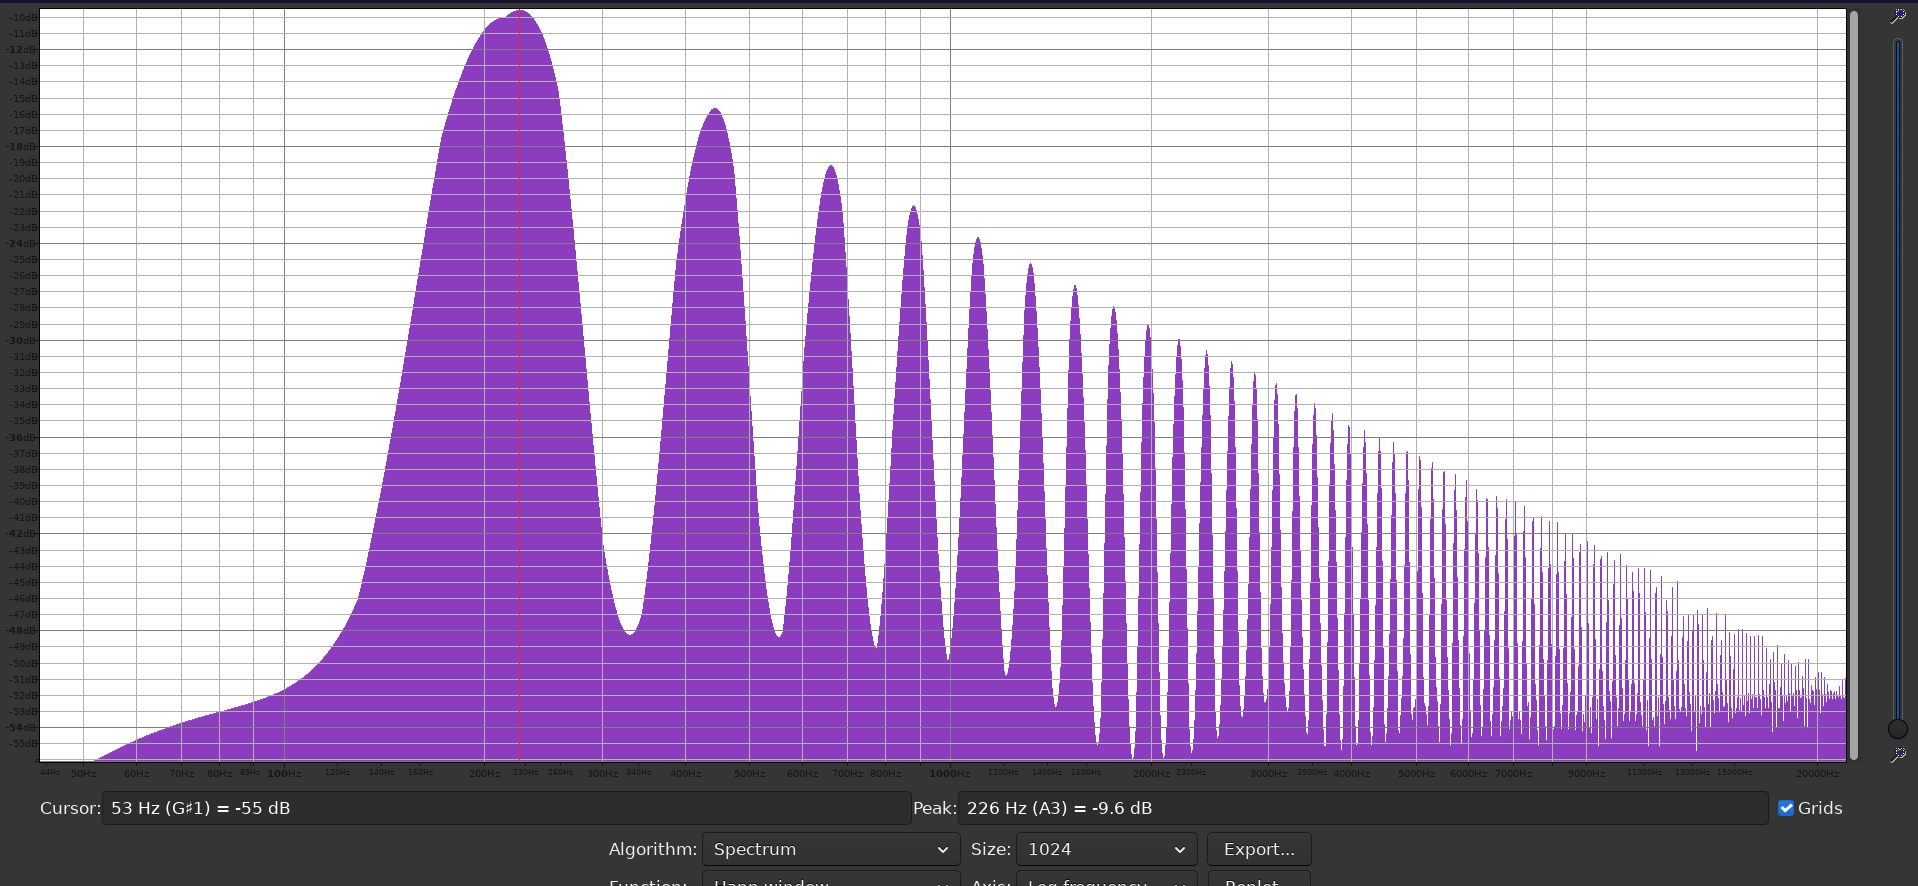
\includegraphics[width=\linewidth]{discussion/synth/figures/saw_spectrum.png}
  \end{minipage}
  \hfill
  \begin{minipage}[b]{0.48\linewidth}
    \centering
    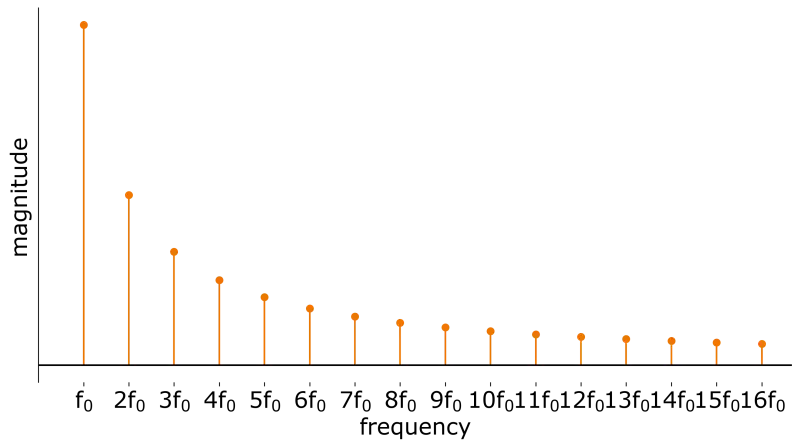
\includegraphics[width=\linewidth]{discussion/synth/figures/sawtooth_harmonics.png}
  \end{minipage}
  \caption{Side-by-side comparison between the frequency spectrum, measured (left) and theoretical (right)}
  \label{fig:saw_spectrum}
\end{figure}

Since the fourier representation of the sawtooth wave is described by the following equation,
\begin{equation}\label{eq:sawtooth_fourier}
    x(t) = \frac{2}{\pi}\sum_{n=1}^{\infty} \frac{(-1)^{n+1}}{n}\sin(2\pi n f_0 t)
\end{equation}

It produces mulitple harmonics with the first peak being the dominant frequency,
followed by an exponential decay by a factor of $\frac{1}{n}$, and contains all the
series of harmonics, for $n \in \mathbb{N}$. After carefully comparing the patterns, 
it is confirmed that the oscillator algorithm behaves as 
expected.
